\documentclass[]{jocg}

\usepackage{amsmath,amsfonts}
\usepackage{amsthm}

\usepackage[utf8]{inputenc}
\usepackage[english]{babel}
\usepackage{booktabs}
\usepackage{mathtools}
\usepackage[mathlines]{lineno}
\usepackage[]{graphicx}
\usepackage{algorithm}
\usepackage[noend]{algpseudocode}
\linenumbers


\setcounter{tocdepth}{1} % -- part,chapters,sections

\usepackage[
  backend=biber,
  style=nature,
  sorting=ynt
]{biblatex}
\addbibresource{main.bib}


\newcommand{\RR}{\mathbb{R}}
\newcommand{\PP}{\mathcal{P}}
\newcommand{\EE}{\mathcal{E}}
\newcommand{\set}[1]{\{#1\}}
\newcommand{\norm}[1]{\|#1\|}
\newcommand{\abs}[1]{|#1|}
\newcommand{\chordarc}{{s_{\abs{\partial~\cdot~}}}}
\DeclareMathOperator{\diam}{\mathrm{diam}}
\DeclareMathOperator{\conv}{\mathcal{}}



\newtheorem{proposition}{Proposition}[section]

\theoremstyle{definition}
\newtheorem{definition}[proposition]{Definition}

\theoremstyle{remark}
\newtheorem{remark}[proposition]{Remark}


\title{%
  \MakeUppercase{Measuring polygonal niceness}%
  \thanks{%
    This paper constitutes the completion of the final project for AMS 545
    ``Computational Geometry''.
  }
}

\author{%
  Sharmila~Duppala%
  \thanks{%
    \affil{Department of Computer Science}, 
    \email{sduppala@cs.stonybrook.edu}%
  }\, and
  David~Kraemer.%
  \thanks{%
    \affil{Department of Applied Mathematics},
    \email{david.kraemer@stonybrook.edu}%
  }
}

\begin{document}

\maketitle

\begin{abstract}
  The $\alpha$-fatness and chord-arc scores as measures of the ``niceness'' of
  polygons are developed and explored, with initial theoretical and empirical
  results. 
\end{abstract}

\tableofcontents

\section{Introduction}

Convexity is from many perspectives the ``gold standard'' of niceness for planar
subsets, because it excludes at once large classes of pathological sets
altogether. Yet for establishing a quantitative measure of niceness that matches
with intuitive or legal understandings, convexity is both too restrictive and too
general. The relevant consideration at present revolves around drawing electoral
districts. The immense political consequences of favorable (or unfavorable)
maps has resulted in the development of creative classes of polygonal regions
utilized for this purpose. There exists a strong civic prerogative for providing
quantitative measures of niceness. In a concurrent opinion in the 2004 suit
\textit{Vieth v. Jubelirer} decided by the U.S. Supreme Court, Justice Anthony
Kennedy writes 
\begin{quote}
  Because, in the case before us, we have no standard by which to measure the
  burden appellants claim has been imposed on their representational rights,
  appellants cannot establish that the alleged political classifications burden
  those same rights.  Failing to show that the alleged classifications are
  unrelated to the aims of apportionment, appellants’ evidence at best
  demonstrates only that the legislature adopted political classifications. That
  describes no constitutional flaw, at least under the governing Fourteenth
  Amendment standard. \cite{2004vieth}
\end{quote}
Ought convexity be considered as such a standard? In practice, convexity is too
restrictive (e.g., for coastal or river borders) and too general (e.g., a tiny
vertical strip) for this purpose.

The aim of this paper is to propose several alternative measures to determine
the niceness of polygonal regions in a quantitatively rigorous way. We introduce
two classes of measures, the $\alpha$-score and the chord-$f$ scores, develop
some of their basic properties, and show how they perform on simulated data. The
$\alpha$-fatness quantifies how much a given polygon resembles a ball (with
respect to some norm). When $f$ measures the perimeter of a polygon, the
chord-$f$ score quantifies the extent to which ``local nonconvexity'' affects
the distribution of the total boundary. Both measures generally reward convex
polygons, but punish certain convex ``offenders.'' Of course, there exist
nonconvex polygons who score well on both measures as well.

This paper proceeds as follows. Section 2 provides a theoretical overview for
the $\alpha$-fatness and chord-$f$ scores and gives preliminary results on
simple examples. Section 3 outlines the algorithms used to perform
discretizations and compute the $\alpha$-fatness and chord-$f$ scores. Section 4
gives the results of numerical simulations for these measures on randomly
generated ``typical'' polygons and provides data about the success of
discretization. Section 5 includes a discussion of the main results of the paper
and its implications for the electoral districting process.

Source code for this project can be found at
\url{https://github.com/DavidNKraemer/polygonal-niceness}. Documentation, cruft
removal, and user interface improvements are presently evolving.

\section{Theoretical background}

The area of a subset $S \subseteq \RR^2$ of the plane is denoted by
$\lambda(S)$. We will denote the boundary of $S$ by $\partial S$. For two points
$x,y \in \RR^2$, the closed line segment with endpoints in $x$ and $y$ is
denoted $[x,y]$. For $p \in [1, \infty]$, we define the $p$-ball as $B_{p}(x,
\varepsilon) = \set{y \in \RR^2 : \norm{x-y}_p \leq \varepsilon}$ and we will
only be interested in the closed case. Unless otherwise stated, we shall operate
in the Euclidean world with $p = 2$. Throughout we shall assume that $P
\subseteq \RR^2$ is a simple bounded closed polygon. The class of such polygons
is given by $\PP$. Its perimeter is denoted by $\abs{\partial P}$.

\subsection{The $\alpha$-fatness score}

One approach to measuring the relative ``fatness'' of a polygon seeks to
identify regions of the shape which behave highly unlike balls.

\begin{definition}
  The $\alpha$-fatness score of a polygon $P$ is given by
  \begin{equation*}
    \alpha(P) = \inf\set{\frac{\lambda[P \cap B(x,
    \varepsilon)]}{\lambda[B(x,\varepsilon)]} : \varepsilon > 0, x \in P}
  \end{equation*}
  where we impose that the ball $B(x,\varepsilon)$
  does not contain $P$. 
  \label{def:alpha}
\end{definition}

The constraint that $P \not\subseteq B(x,\varepsilon)$ ensures definiteness:
otherwise, let $\varepsilon \to \infty$ and the ratio $\frac{\lambda[P \cap B(x,
\varepsilon)]}{\lambda[B(x, \varepsilon)]}$ always approaches $0$. An intuition
for $\alpha(P)$ emerges from considering how it behaves on balls.

\begin{proposition}
  For any $P$, $\alpha(P) \leq \frac{1}{4}$, and if $P = B(x_0, r)$
  then we have equality.
  \label{prop:alpha}
\end{proposition}

\begin{proof}
  To show that $\alpha(P) \leq \frac{1}{4}$, it suffices to show only for convex
  $P$, because $P \subseteq \conv(P)$ implies $\lambda[P \cap B(x, \varepsilon)]
  \leq \lambda[\conv(P) \cap B(x, \varepsilon)]$. Let $d = \diam (P)$ and fix
  $x,y \in \partial P$ such that $\abs{[x,y]} = d$. Assume without loss of
  generality that $x$ lies above $y$, and consider the ball $B(x, d)$. Then $P$
  does not meet the upper disk of $B(x,d)$, for otherwise we could choose $z \in
  P$ in the upper disk of $B(x,d)$ which forms a chord of $P$ longer than $d$.
  A similar argument shows that $P$ cannot occupy more than half of the lower
  disk of $B(x,d)$. Hence
  \begin{equation*}
    \alpha(P) \leq \frac{\lambda[P \cap B(x,d)]}{\lambda[B(x,d)]} \leq
    \frac{1}{4},
  \end{equation*}
  as needed.

  The fact that $\alpha(B(x_0, r)) = \frac{1}{4}$ relies on a neat
  result \cite{10.2307/30044198} that shows that the $L_p$
  ellipsoid $\EE$ with radii $a, b$ has area
  \begin{equation*}
    \lambda(\EE) = a b \cdot 4
    \frac{\Gamma(1+\frac{1}{p})^2}{\Gamma(1+\frac{n}{p})}.
  \end{equation*}
  In our case, $\alpha(B(x_0, r))$ is achieved at a ball on a ``corner'' point
  with radius $2r$.
\end{proof}

Hence, the $\alpha$-score is greater for polygons which exhibit ``niceness''
characteristics. It is not affected tremendously by local nonconvexity in $P$ so
long as $P$ ``snugly fits'' into a ball shape, which is a global property.

\subsection{The chord-$f$ score}

A different class of ``fatness'' measures arises through partitioning $P$ into
two (interior disjoint) polygons $P = P' \cup P''$ via chords. A chord is a pair
$x,y \in \partial P$ such that the segment $[x,y]$ is contained in the interior
of $P$ except at the endpoints $x$ and $y$. Such a chord defines a partition of
$P = P' \cup P''$ by orientation, so that $\partial P'$ is the arc from $x$ to
$y$ together with $[x,y]$ and that $\partial P''$ is the arc from $y$ to $x$
together with $[x,y]$.

\begin{definition}
  Let $f : \mathcal{P} \to \RR$. For a given $P \in \mathcal{P}$, its
  \emph{chord-$f$ score} is given by
  \begin{equation*}
    s_f (P) = \inf \set{\max(f(P'), f(P'')) : x, y \in \partial P}
  \end{equation*}
  where the chord $[x,y]$ partitions $P = P' \cup P''$.
  \label{def:chord-f}
\end{definition}

The intuition for $f$ is some global measure of ``cost'' associated with respect
to $P$. For example, if $f(P) = \abs{\partial P}$, then $s_f$ identifies the
partition (or limiting sequence of partitions) which minimizes the maximum
subpolygon perimeter. Indeed, measures such as perimeter or area are the typical
choices of $f$, but any suitable property of $P$  may be employed. 

The chord-$f$ score can be understood relatively simply in the context of a
minimax game. Max, given a polygon with a chord partitioning it, always chooses
the subpolygon associated with a greater $f$ (i.e., the worst cost of the
partition). Min, who plays first, tries to find a chord with the least-bad worst
cost with respect to $f$.

The member of this class of scores under this present investigation is
$\chordarc$, the so-called \emph{chord-arc} score. It is important to note that
the length of the chord $[x,y]$ which partitions $P$ is included in the
estimation of $\chordarc$. One implication of this is that the chord-arc score
need not be bounded above by $\frac{\abs{\partial P}}{2}$.  We have several
facts about $\chordarc$ which develop further intuition for the score.
\begin{proposition}
  \begin{enumerate}
    \item Let $R$ be a rectangle with height $h$ and length $\ell$. Assume that
      $h \leq \ell$. Then $\chordarc(R) = 2h + \ell$.
    \item Let $P$ be convex with perimeter $\abs{\partial P} = w$. Then
      $\chordarc(P) \leq \frac{w}{2} + \diam (P)$.
    \item Let $C$ be a circle with ``perimeter'' $2\pi r$. Then $\chordarc(C) =
      (\pi + 2)r$.
  \end{enumerate}
  \label{rem:chordarc}
\end{proposition}

\begin{proof}
  \begin{enumerate}
    \item That the optimal partition bisects $R$ is readily apparent,
      for this minimizes the maximum perimeter length of either sub-rectangle.
      A case analysis confirms that the preferred strategy for Min is to choose
      a chord along the smaller dimension (i.e., $h$) to bisect $R$, and in this
      case the maximum arc length is $2h + 2\left( \frac{\ell}{2} \right) = 2h +
      \ell$, as needed.
    \item For $P$ convex, a perimeter-bisecting chord, whose length is at most
      $\diam(P)$, always exists. 
    \item This follows from part 2 by noticing that the length of \emph{any}
      perimeter-bisecting chord is $\diam(C) = 2r$. \qedhere
  \end{enumerate}
\end{proof}

\section{Overview of empirical design}

In principal of computing the $\alpha$ and chord-$f$ scores relies on sweeping
the continuum of points of $P$ and evaluating the aforementioned measurements.
To estimate this process in practice, we employ the following discretizing
scheme. Let $P$ be determined by the vertices $[v_1, \dots, v_n]$ given in
counterclockwise order. Then, given $\delta > 0$, loop through the vertices of
$P$, checking if $\norm{v_{i+1} - v_i} > \delta$. In the case where this holds,
we insert $v_i' = \frac{v_i + v_{i+1}}{2}$ after $v_i$ into the polygon and
resume the loop. This ensures that for any two adjacent vertices $v_{i}$ and
$v_{i+1}$ in the representation of $P$ we have $\norm{v_{i+1} - v_i} \leq
\delta$. As $\delta \to 0$ this estimates $\partial P$ more exactly. All
computations are done with respect to the $L_{\infty}$ norm. The implementation
of this procedure is given in Algorithm \ref{alg:delta}.

Depending on the relative coordinates of the vertex set compared to $\delta$,
the worst-case runtime of refinement varies. In the case where the maximum
distance is $\delta K$, the refinement adds $O(\lg^2 K)$ vertices between the
two coordinates. The overall runtime is $O(n \lg^2 K)$ and the total quantity of
vertices after refinement is $O(n + n\lg^2 K)$.

%% Pseudocode for the delta refinement

\begin{algorithm}[h]
  \begin{algorithmic}[1]
    \Procedure{RefineBy}{$P,\delta$}
    \State{$P = [v_1, v_2, v_3, \dots, v_n]$};
    \State{$v = v_1$}
    \While {$\textit{next}(v) \ne v_1$}
    \If {$\norm{\textit{next}(v) - v}_2 > \delta$} 
      \State{\textrm{Insert $\textit{midpoint}(v, \textit{next}(v))$ into $P$ after $v$}} 
      \Comment{Now $\textit{next}(v)$ is the midpoint}
    \EndIf
    \EndWhile
    \EndProcedure
  \end{algorithmic}
  \caption{%
    The procedure used to refine a given polygon $P$ by a specified $\delta >
    0$. This modifies the existing $P$ to satisfy the regularity condition
    that $\norm{v_{i+1} - v_i} \leq \delta$ for each adjacent vertex pair
    $v_{i+1}, v_i$ on the discretized boundary $\partial P$.  }
  \label{alg:delta}
\end{algorithm}

Given a $\delta$-refined polygon $P$, the computation of $\alpha(P)$ is
relatively straightforward, with the simplification that points $x$ on which the
ratio is computed lie on $\partial P$. The computation steps through $[v_1,
\dots, v_n]$ and for each $v_i$ the radius $\varepsilon$ of the
minimum-enclosing $\infty$-ball centered at $v_i$ is computed. Then for
$\varepsilon_k = \frac{k}{100} \varepsilon$, $k = 1, \dots, 100$, the ratio 
\begin{equation*}
  \frac{\lambda[P \cap B_{\infty}(v_i, \varepsilon_k)]}{B_{\infty}(v_i,
  \varepsilon_k)}
\end{equation*}
is computed and the smallest such ratio is kept. The minimum over all $v_i$ is
given as $\alpha(P)$. The implementation of the $\alpha$ score is given in
Algorithm \ref{alg:alpha}. Though we use a sweep from $k = 1, \dots, 100$, any
suitable range may be selected as an alternative. Unfortunately, there is no
analogous ``bisection'' technique for determining the minimizing $k$ because
this ratio need not be monotonic. Since $P$ need not be convex, the intersection
$P \cap B_{\infty}(v, \varepsilon_k)$ requires $O(n \log n)$ steps. For $n$
vertices, the runtime performance is $O(n^2 \log n)$.

%% Pseudocode for the alpha score

\begin{algorithm}[h]
  \begin{algorithmic}[1]
    \Function{$\alpha$Score}{$P$}
    \State{$P = [v_1, v_2, v_3, \dots, v_n]$};
    \State{$\textrm{min} = \infty$}
    \For {$v \in P$}
    \State{$\varepsilon = \textrm{radius of minimum enclosing ball of $P$ at
    $v$}$}
    \For {$k = 1, 2, \dots, 100$} \Comment{$100$ is arbitrary}
    \State{$\varepsilon_k = \frac{k}{100} \varepsilon$}
    \State{$\textrm{area} = \frac{\lambda[P \cap B_{\infty}(v, \varepsilon_k)]}{B_{\infty}(v, \varepsilon_k)}$}
    \If {$\textrm{min} > \textrm{area}$}
    \State{$\textrm{min} = \textrm{area}$}
    \EndIf
    \EndFor
    \EndFor
    \State{\Return{\textrm{min}}}
    \EndFunction
  \end{algorithmic}
  \caption{%
    The $\alpha$-fatness function.  }
  \label{alg:alpha}
\end{algorithm}

Similarly, given a $\delta$-refined polygon $P$, the chord-$f$ score is computed
by sweeping all possible chords of $P$. For each point $v_i, v_j \in \partial P$
with $i < j$, if $[v_i, v_j]$ is indeed a valid chord of $P$, the partition $P =
P' \cup P''$ is computed and the maximum of $f(P')$ and $f(P'')$ is kept. The
minimum such value is given as $s_f(P)$. The implementation of the chord-$f$
score is given in Algorithm \ref{alg:chordf}. For $n$ vertices, $O(n^2)$
potential chords are computed. To determine if a pair of vertices is a chord
takes $O(n)$ time, which leads to an overall runtime performance of $O(n^3)$.


%% Pseudocode for the chord f score

\begin{algorithm}[h]
  \begin{algorithmic}[1]
    \Function{ChordScore}{P,f}
    \State{$P = [v_1, v_2, v_3, \dots, v_n]$};
    \For {$v \in P$}
    \For {$w \in [\textit{next}(v), \dots, v_n]$}
    \If {$[v,w]$ is a chord of $P$}
      \State{Partition $P = P' \cup P''$ by $[v,w]$}
      \State{$\textrm{submax} = \textit{max}(f(P'), f(P''))$}
      \If {$\textrm{min} > \textrm{submax}$}
        \State{$\textrm{min} = \textrm{submax}$}
      \EndIf
    \EndIf
    \EndFor
    \EndFor
    \State{\Return{\textrm{min}}}
    \EndFunction
  \end{algorithmic}
  \caption{%
    The chord-$f$ function.   }
  \label{alg:chordf}
\end{algorithm}

All of these algorithms are implemented in CGAL \cite{cgal:eb-18a} with the
extensive use of the 2D Polygon library \cite{cgal:gw-p2-18a}. For our data
generation, we make the minor modification that measured ${\chordarc}$ is the
ratio of the actual $\chordarc$ score with the perimeter of the overall polygon.
This changes the interpretation of some of the theoretical results from the
previous section but allows for easier interpretation of the data.

\section{Empirical results}

We evaluate our measurements on randomly generated polygons with vertices in the
unit square $[0,1] \times [0,1]$. We consider collections of such polygons of
10, 50, and 100 vertices. In Figure \ref{fig:delta-alpha} and Figure
\ref{fig:delta-arc}, we measure the effect on
polygons of 10 vertices of sweeping $\delta$ between $0.05$ and $1$ on the
resulting measurements. Figure \ref{fig:alph-inft-10} shows a comparison of
$\alpha$-fatness and relative ${\chordarc}_{\infty}$ scores for polygons on 10
vertices.  Figure \ref{fig:alph-one-50} shows a comparison of $\alpha$-fatness
and relative ${\chordarc}_1$ scores for polygons on 50 vertices. Figure
\ref{fig:alph-inft-100} shows a comparison of $\alpha$-fatness and relative
${\chordarc}_{\infty}$ scores for polygons on 100 vertices.

Our theoretical results seem to be confirmed in that ``ball''-like polygons get
the highest $\alpha$-scores, and it seems that polygons with fewer
``nonconvexities'' score better on the relative ${\chordarc}_{\infty}$ measure. We
observe an overall decline in the relative $\chordarc$ scores as the number of
vertices of the polygons increases. This is attributed to the corresponding
increase in the size of the underlying perimeters of each $P$. The observation
is not shared with the $\alpha$ score, but this can be understood as a sort of
``coastline'' phenomenon, in which polygonal perimeters increase without limit
while the areas converge.


\begin{figure}[t]
  \centering
  \begin{tabular}{lrrrrrrrrrr}
    \toprule
    $\delta$ & 1 & 2 & 3 & 4 & 5 & 6 & 7 & 8 & 9 & 10 \\
    \midrule
    0.05 &  0.23 &  0.21 &  0.11 &  0.039 &  0.15 &  0.038 & 0.12 &  0.10 &  0.12 &  0.13 \\
    0.15 &  0.23 &  0.21 &  0.11 &  0.039 &  0.15 &  0.038 & 0.12 &  0.10 &  0.12 &  0.13 \\
    0.26 &  0.23 &  0.21 &  0.11 &  0.039 &  0.15 &  0.038 & 0.12 &  0.10 &  0.12 &  0.13 \\
    0.36 &  0.23 &  0.21 &  0.11 &  0.039 &  0.15 &  0.038 & 0.12 &  0.10 &  0.12 &  0.13 \\
    0.47 &  0.23 &  0.21 &  0.11 &  0.039 &  0.15 &  0.038 & 0.12 &  0.10 &  0.12 &  0.13 \\
    0.57 &  0.23 &  0.21 &  0.11 &  0.039 &  0.15 &  0.038 & 0.12 &  0.10 &  0.12 &  0.13 \\
    0.68 &  0.23 &  0.21 &  0.11 &  0.039 &  0.15 &  0.038 & 0.12 &  0.10 &  0.12 &  0.13 \\
    0.78 &  0.23 &  0.21 &  0.11 &  0.039 &  0.15 &  0.038 & 0.12 &  0.10 &  0.12 &  0.13 \\
    0.89 &  0.23 &  0.21 &  0.11 &  0.039 &  0.15 &  0.038 & 0.12 &  0.10 &  0.12 &  0.13 \\
    1    &  0.23 &  0.21 &  0.11 &  0.039 &  0.15 &  0.038 & 0.12 &  0.10 &  0.12 &  0.13 \\
    \bottomrule
  \end{tabular}
  \caption{%
    Effect of sweeping $\delta$ on measurements of $\alpha$-score on
    10 randomly generated polygons with 10 vertices in $[0,1]^2$.
    Unsurprisingly, the refinement of the different polygons has no effect on
    the $\alpha$-fatness score, since it introduces no additional area to the
    polygon and since the ``corners'' are already present.
  }
  \label{fig:delta-alpha}
\end{figure}

\begin{figure}[t]
  \centering
  \begin{tabular}{lrrrrrrrrrr}
    \toprule
    $\delta$ & 1 & 2 & 3 & 4 & 5 & 6 & 7 & 8 & 9 & 10 \\
    \midrule
    0.05  &  0.83 &  0.46 &  0.83 &  0.89 &  0.54 &  0.67 &  0.62 &  1.00 &  0.86 &  0.55 \\
    0.15  &  0.79 &  0.90 &  0.72 &  0.60 &  0.90 &  0.67 &  0.99 &  0.83 &  0.66 &  0.90 \\
    0.26  &  1.00 &  0.75 &  0.50 &  0.60 &  0.90 &  0.49 &  0.77 &  0.52 &  0.72 &  0.69 \\
    0.36  &  0.89 &  1.00 &  0.50 &  0.60 &  0.52 &  0.49 &  1.00 &  0.92 &  0.74 &  0.51 \\
    0.47  &  0.61 &  1.00 &  0.50 &  0.75 &  0.52 &  0.24 &  1.00 &  0.62 &  1.00 &  0.51 \\
    0.57  &  0.61 &  1.00 &  0.25 &  0.75 &  0.52 &  0.24 &  1.00 &  0.62 &  1.00 &  0.51 \\
    0.68  &  0.61 &  1.00 &  0.25 &  0.75 &  0.52 &  0.24 &  1.00 &  0.62 &  1.00 &  0.51 \\
    0.78  &  0.61 &  1.00 &  0.25 &  0.75 &  0.52 &  0.24 &  1.00 &  0.62 &  1.00 &  0.51 \\
    0.89  &  0.61 &  1.00 &  0.25 &  0.75 &  0.52 &  0.24 &  1.00 &  0.62 &  1.00 &  0.51 \\
    1     &  0.61 &  1.00 &  0.25 &  0.75 &  0.52 &  1.00 &  1.00 &  0.62 &  1.00 &  0.51 \\
    \bottomrule
  \end{tabular}
  \caption{%
    Effect of sweeping $\delta$ on measurements of ${\chordarc}_\infty$ on
    10 randomly generated polygons with 10 vertices in $[0,1]^2$. The overall behavior is
    difficult to summarize.  Though one might hope that as $\delta \to 0$ we see
    a stabilization in the chard arc score, this does not appear to occur.
    Moreover, there does not seem to be even a monotonic evolution in the score
    as $\delta \to 0$. This is likely due to the fact that smaller values of
    $\delta$ permit stranger nonconvexities to emerge as viable chords.
  }
  \label{fig:delta-arc}
\end{figure}

\begin{figure}[t]
  \centering
  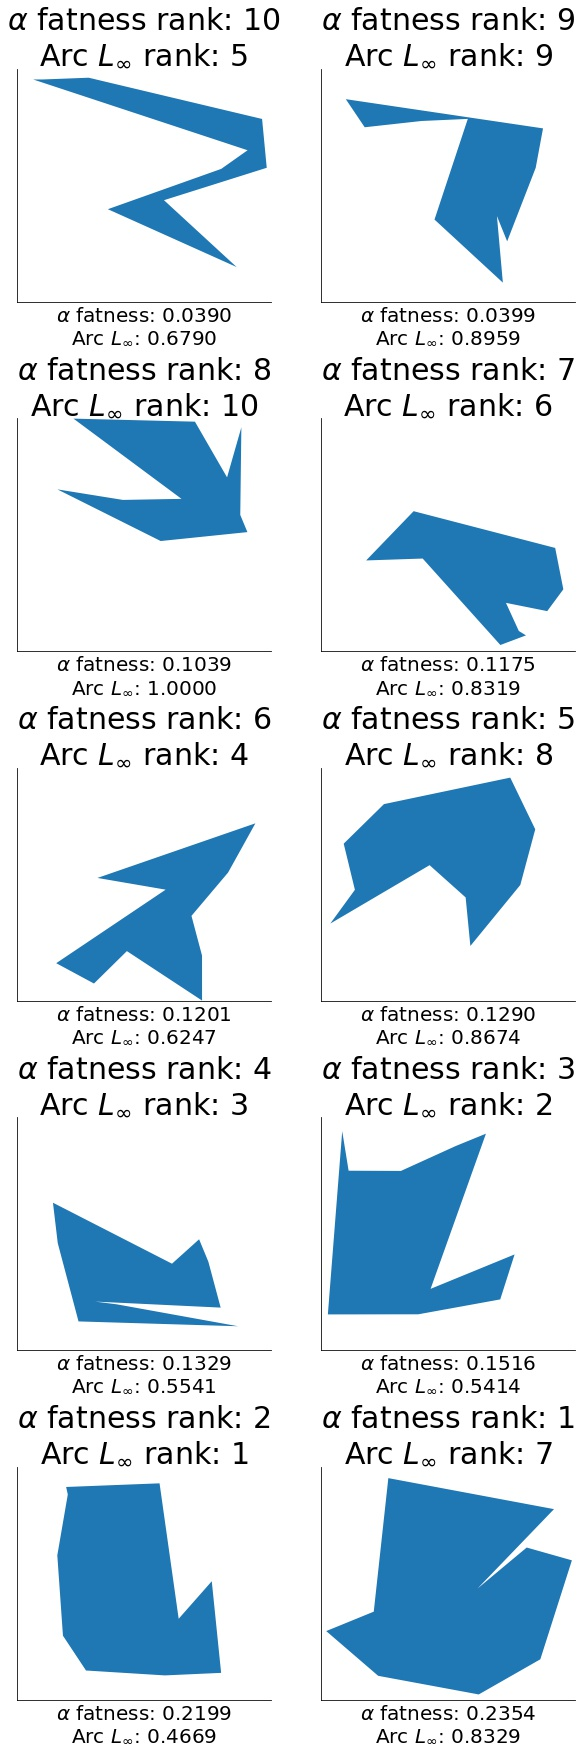
\includegraphics[height=0.8\textheight]{../plots/u_10_alpha_score_chord_arc_infinity_vertices_0-05_delta_ranking.jpg}
  \caption{$\alpha$ scores and ${\chordarc}_{\infty}$ scores for randomly
  generated polygons on 10 vertices.}
  \label{fig:alph-inft-10}
\end{figure}

\begin{figure}[t]
  \centering
  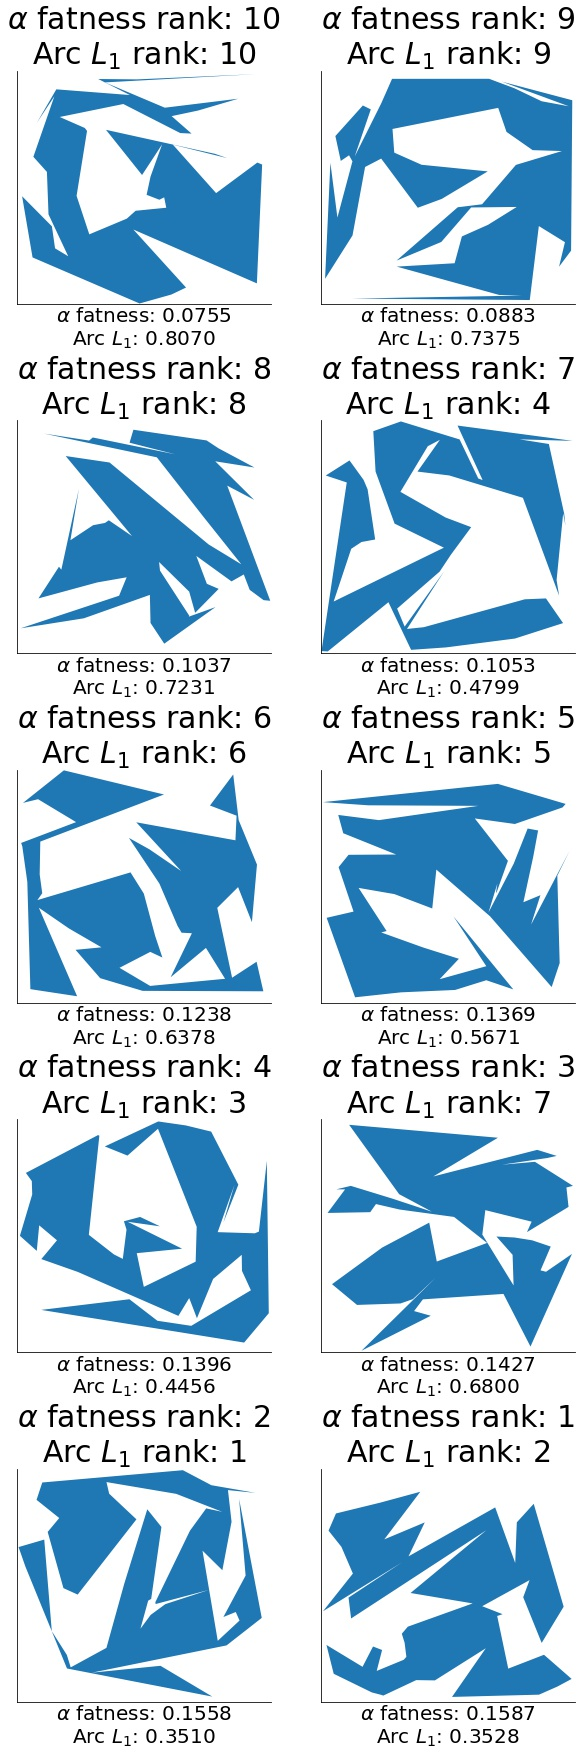
\includegraphics[height=0.8\textheight]{../plots/u_50_alpha_score_chord_arc_one_vertices_0-05_delta_ranking.jpg}
  \caption{$\alpha$ scores and ${\chordarc}_{1}$ scores for randomly
  generated polygons on 50 vertices.}
  \label{fig:alph-one-50}
\end{figure}

\begin{figure}[t]
  \centering
  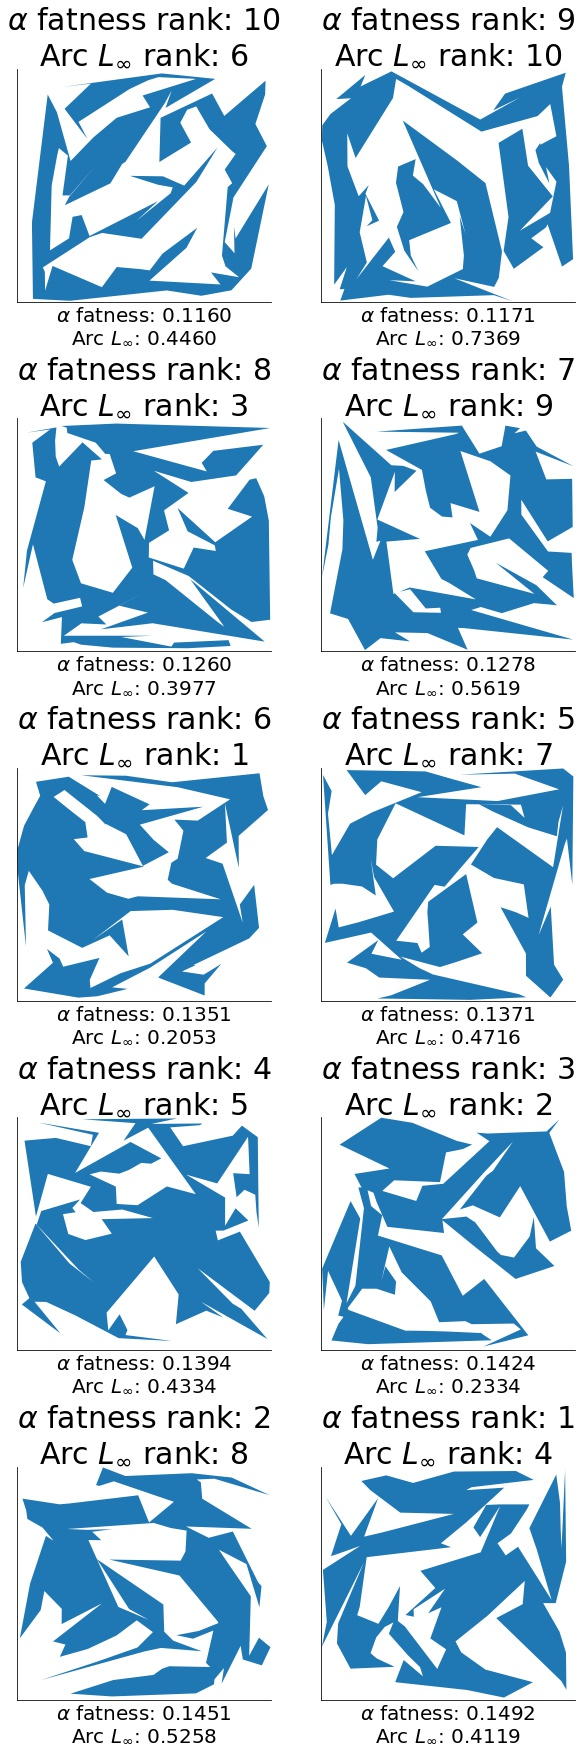
\includegraphics[height=0.8\textheight]{../plots/u_100_alpha_score_chord_arc_infinity_vertices_0-05_delta_ranking.jpg}
  \caption{$\alpha$ scores and ${\chordarc}_{\infty}$ scores for randomly
  generated polygons on 100 vertices.}
  \label{fig:alph-inft-100}
\end{figure}

\section{Discussion}

We have developed two classes of measurements for determining the niceness of
polygonal regions in the plane and established initial results, both theoretical
and empirical, for evaluating their effectiveness. The $\alpha$-fatness measures
the extent to which the underlying polygon resembles a ball. It rewards
polygons which fill squarely compact regions and punishes oblong and spread out
polygons. The chord-arc score measures the extent to which the underlying
polygon contains significant ``local nonconvexities'' that are not well
distributed throughout the entire polygon. Interestingly, both measures perform
well (even optimally) on specific types of convex polygons but severely punishes
others. We generally find that these measures conform in some sense to an
intuitive understanding of niceness.

Extensions on these measures can be examined. The connected $\alpha$-fatness
score, for example, computes the intersection of $B(x,\varepsilon)$ with the
connected component of $P$ containing $x$. This might prove a more reliable
estimate of intuitive niceness than the conventional $\alpha$-fatness score,
because it excludes components of $P$ from consideration which are close in a
coarse sense, but not necessarily close in a topological sense. The myriad of
possible choices from which to choose $f$ leaves open a wide space for
exploration. A more suitable measure than simply the perimeter may emerge as a
consequence.

The next extension of this work is to apply these measures to electoral
districts and evaluate their success at distinguishing between offending and
``nice'' districts. Given an increasing corpus of election districts ruled out
or struck down by constitutional grounds, it may be possible to learn a
classification model using these measures. Alternatively, it may be discovered
that these measures are sufficient to distinguish between offending and nice
districts in an unsupervised fashion.

Whether quantitative measures that conform to intuitive understandings of
niceness is relevant to crafting electoral districts at all remains an open
question. General compactness and contiguity are only part of the requirements
which an electoral district must satisfy under the present regime, whereas
others, such as those given in the 1965 Voting Rights Act, bear less consequence
from the pure shape of the district. Doubtless these quantitative measures could
form part of the evaluation process for determining new districts, but the
actual policy will almost surely involve ensembles of measures, both
quantitative and otherwise, in idealized future redistricting.


\printbibliography[heading=bibintoc]

\end{document}
